\section{Экспериментальная часть}
\subsection{Эксперимент по проверке точности измерения времени}
Для проверки точности измерения времени проведём следующий эксперимент.

Сгенерируем семейство программ, которые не делают ничего, кроме вызова функции стандартной библиотеки \textit{C} \textit{usleep}. Аргументами функции будет число $10^n$, где $n$ --- число от одного до шести включительно. Таким образом, после запуска программа устанавливает таймер на заданное число микросекунд (от 1 мкс до 1000000 мкс = 1 с), останавливается и после его срабатывания завершает работу.

Далее на рис. \ref{img:calibration} приведён график измеренного времени исполнения семейства таких программ и «реального» времени их выполнения --- т.е. времени, указанного в аргументе функции, создающей таймер. График построен с помощью инструментария в автоматическом режиме.

\begin{figure}[p]
    \center{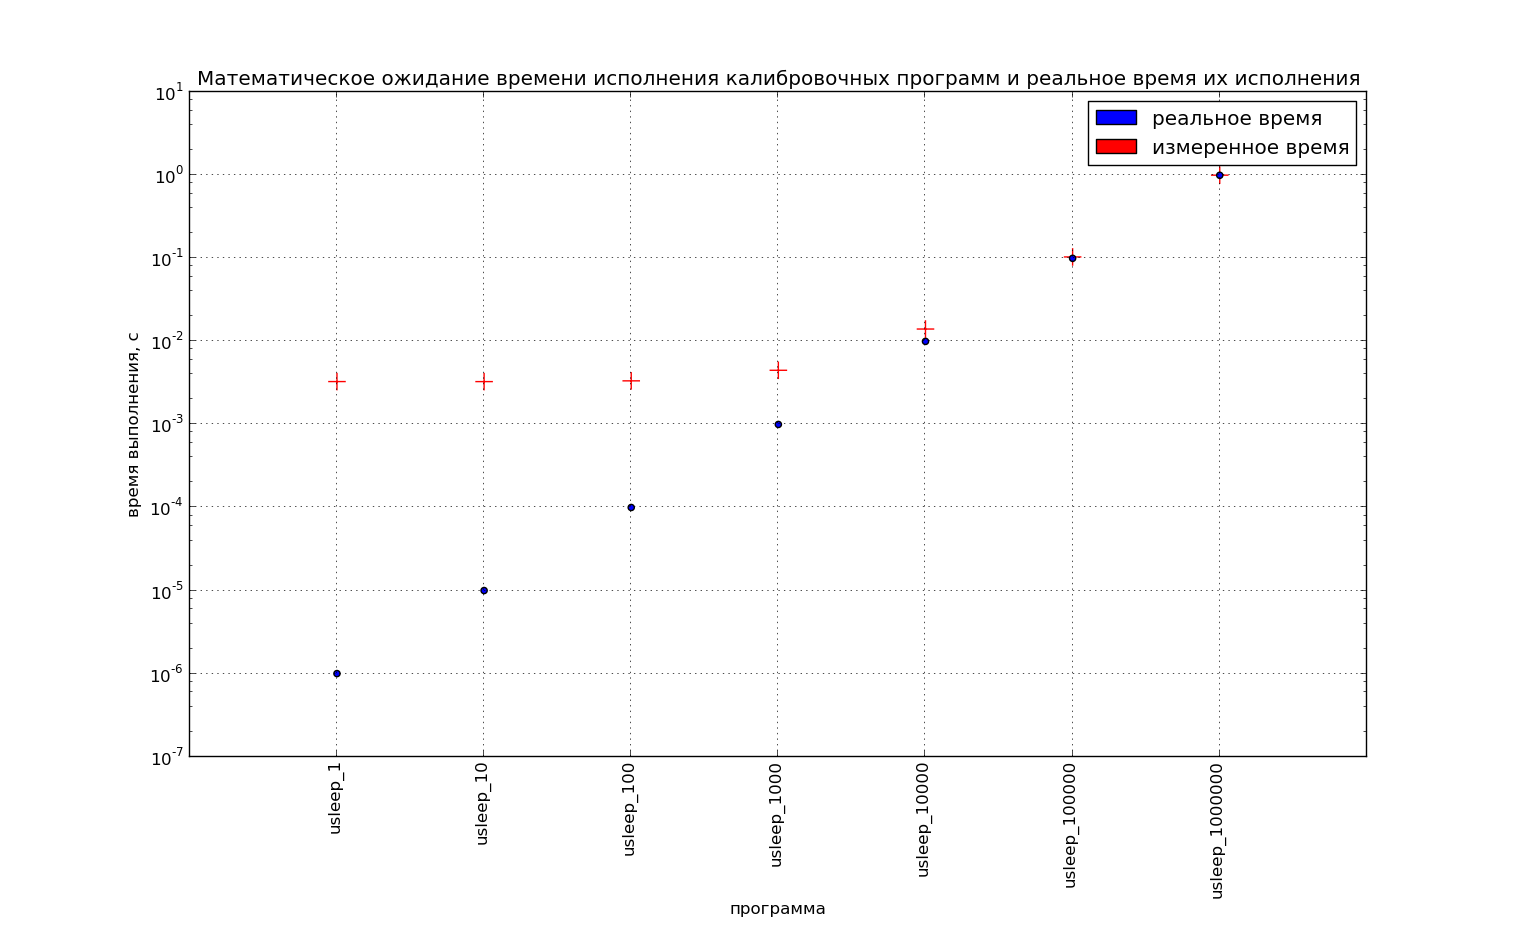
\includegraphics[width=1\linewidth]{calibration}}
    \caption{График измеренного и реального времени исполнения семейства калибровочных программ}
    \label{img:calibration}
\end{figure}

Как мы видим на рис. \ref{img:calibration}, измеренное время асимптотически приближается к значению между $10^{-2}$ и $10^{-3}$ --- около 0,005.

Из этого можно сделать вывод, что существуют постоянные расходы на запуск программы из нашей системы и их можно вычесть из измеренного времени для повышения точности измерения. Для этого мы вычисляем время выполнения пустой программы (согласно описанной в подразделе~\ref{sssect:calibration} методике), а затем вычитаем его из каждого измеренного результата выполнения реальных программ.

На рис. \ref{img:calibration-offset} показан график измеренного времени в данном эксперименте с учётом накладных расходов.

\begin{figure}[p]
    \center{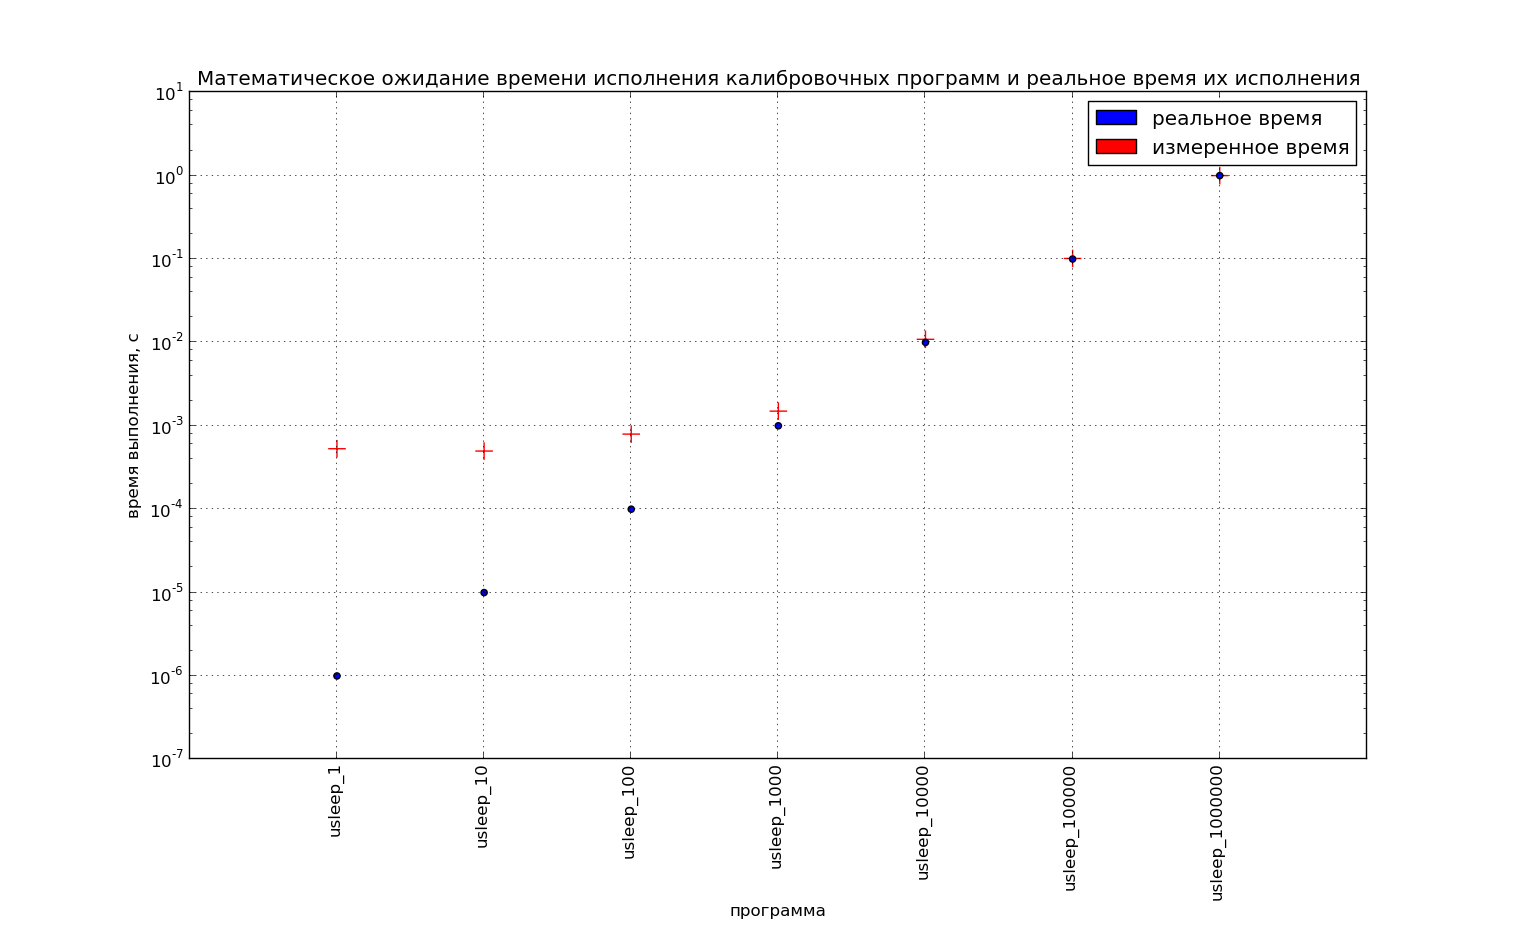
\includegraphics[width=1\linewidth]{calibration-offset}}
    \caption{График измеренного и реального времени исполнения семейства калибровочных программ с учётом накладных расходов}
    \label{img:calibration-offset}
\end{figure}

Далее на рис. \ref{img:default_calibration} приведён текстовый вывод из инструментария результата описанного эксперимента с учётом накладных расходов.

\begin{figure}[H]
    \fontsize{10}{12}
    \begin{verbatim}
        Experiment performed:
            Real time: 0.000001
            Measured time: 0.000531
            Relative error: 530.11
        
        Experiment performed:
            Real time: 0.000010
            Measured time: 0.000498
            Relative error: 48.79
        
        Experiment performed:
            Real time: 0.000100
            Measured time: 0.000795
            Relative error: 6.95
        
        Experiment performed:
            Real time: 0.001000
            Measured time: 0.001499
            Relative error: 0.50
        
        Experiment performed:
            Real time: 0.010000
            Measured time: 0.010893
            Relative error: 0.09
        
        Experiment performed:
            Real time: 0.100000
            Measured time: 0.101603
            Relative error: 0.02
        
        Experiment performed:
            Real time: 1.000000
            Measured time: 1.001015
            Relative error: 0.00
    \end{verbatim}
    \caption{Результат работы программы для описанного выше эксперимента.}
    \label{img:default_calibration}
\end{figure}

Таким образом, инструментарий позволяет производить достаточно точное измерение времени (ошибка в пределах 10\%) для программ, исполняющихся 10 мс и более.


\subsection{Эксперимент по сравнению компиляторов GCC и LLVM на тестовом наборе Polybench}
На рис. \ref{img:gcc-vs-clang} сравнивается время исполнения программ, собранных компиляторами GCC и LLVM соответственно на уровне оптимизации '-O2'. Компилятор на этом уровне оптимизации в подавляющем большинстве случаев генерирует наиболее быстрый код (относительно уровней '-O0' и '-O1').

\begin{figure}[!bH]
    \center{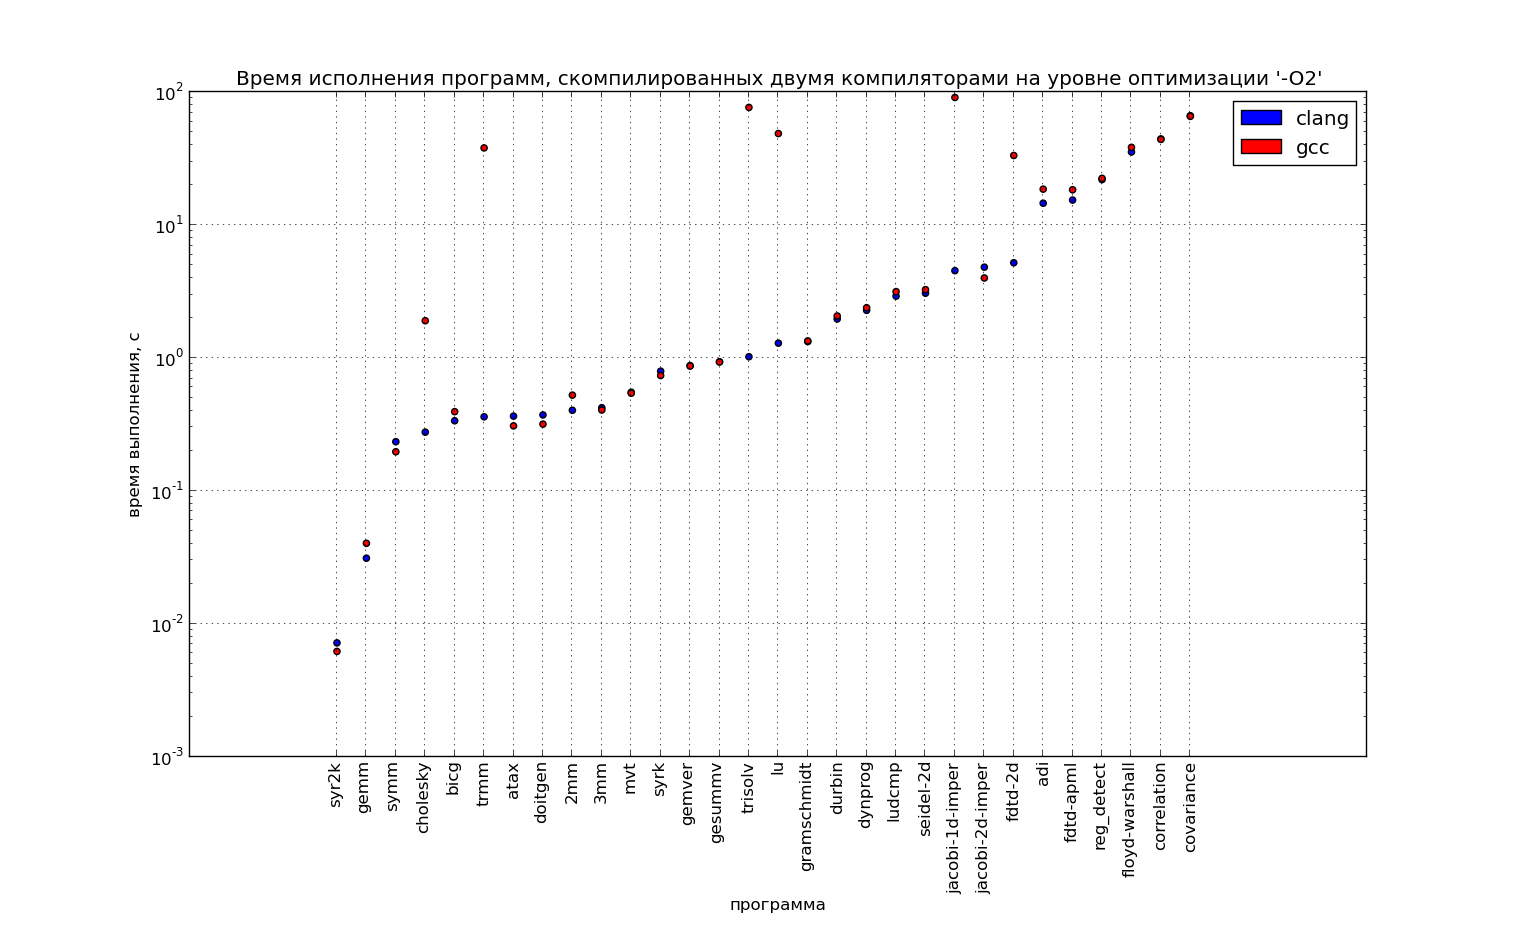
\includegraphics[width=1\linewidth]{gcc-vs-clang}}
    \caption{График времени исполнения программ из набора Polybench для двух компиляторов.}
    \label{img:gcc-vs-clang}
\end{figure}

Как мы видим из графика, на большинстве программ оба компилятора показывают примерно одинаковую производительность. Однако на шести программах компилятор LLVM серьёзно превосходит GCC. Вероятно, LLVM использует лучший векторизатор кода, что оказывает большое влияние в этих специфических случаях. Конкретные причины этого превосходства будут выяснены в дальнейшей работе.